
This chapter defines the IMF language. Further, it introduces the Aspect Object that is central in the creation of IMF models and shows the capabilities of
the language through the creation of Breakdowns and Topologies. \autoref{tab:Table 3} gives an overview of the different terms that
is convenient to have when reading the chapter.  contains the combined diagram of the structural diagrams given
throughout this section. The vocabulary and grammar of the IMF language is implemented using semantic web
technologies, see \autoref{ch:Appendix D}. A
mapping of the IMF vocabulary into first-order logic suitable for developing a translation into ontologies such as
ISO 15926-14 is found in \autoref{ch:Appendix E}.

\begin{table}[htb]
  \centering
  \caption{An overview of terms and symbols in the IMF language.}\label{tab:Table 3}

  \begin{supertabular}{|m{0.50105983in}m{0.53305984in}|m{1.3434598in}|m{1.4253598in}|m{1.4218599in}|m{1.2892599in}|}
    \hhline{-----~}
    \multicolumn{2}{|m{1.11286in}|}{\centering{\bfseries Element}} &
    {\centering Block}

    \centering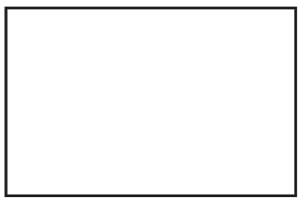
\includegraphics[width=0.73013in,height=0.49152in]{img/IMFmanual-img012.png}  &
    {\centering Terminal}

    \centering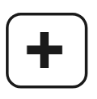
\includegraphics[width=0.23622in,height=0.2411in]{img/IMFmanual-img013.png}  &
    {\centering Association Point}

    \centering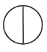
\includegraphics[width=0.21211in,height=0.23767in]{img/IMFmanual-img014.png}  &
    \multicolumn{1}{m{1.2892599in}}{}\\\hhline{-----~}
    \multicolumn{5}{m{5.5397596in}}{} &
    \multicolumn{1}{m{1.2892599in}}{}\\\hline
    \multicolumn{2}{|m{1.11286in}|}{\centering \textbf{Relation}} &
    {\centering hasTerminal}

    \centering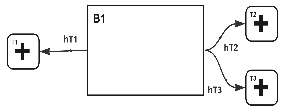
\includegraphics[width=1.26374in,height=0.47837in]{img/IMFmanual-img015.jpg}  &
    {\centering connectedTo}

    \centering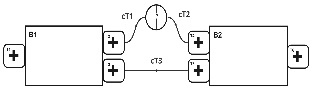
\includegraphics[width=1.34722in,height=0.40972in]{img/IMFmanual-img016.jpg}  &
    {\centering interAspect}

      {\centering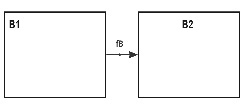
\includegraphics[width=1.06528in,height=0.45139in]{img/IMFmanual-img017.jpg} }
    \centering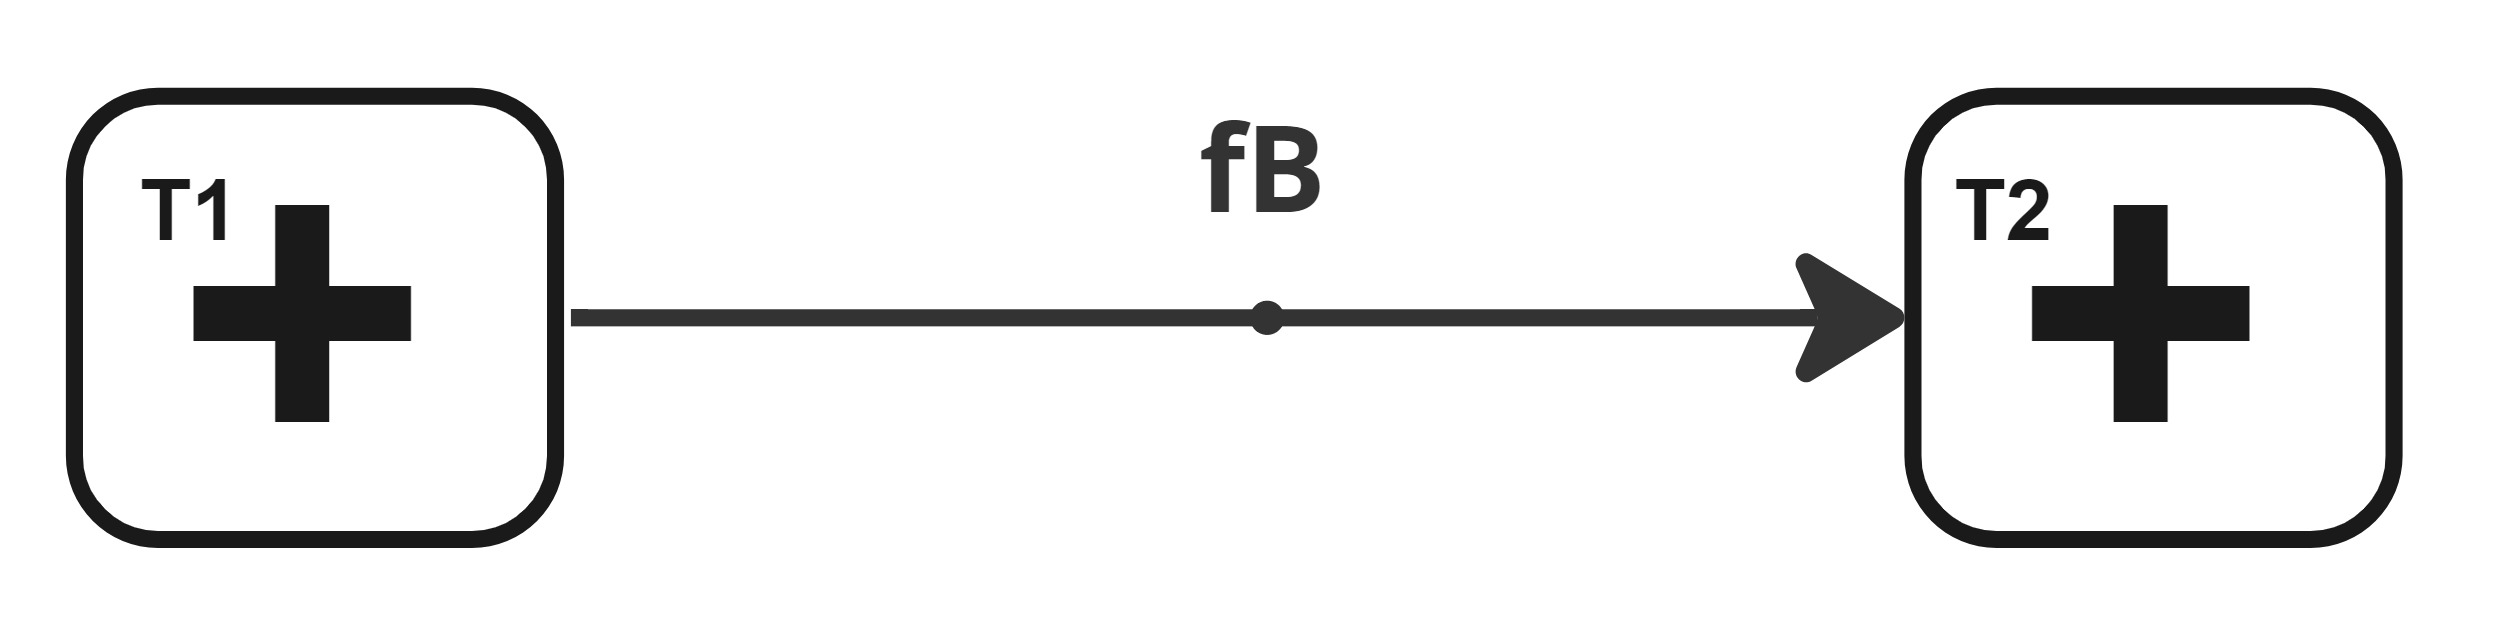
\includegraphics[width=0.91667in,height=0.2277in]{img/IMFmanual-img018.jpg}  &
    {\centering partOf}

    \centering\arraybslash  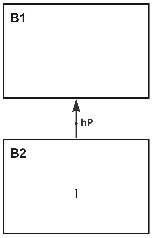
\includegraphics[width=0.68952in,height=1.06587in]{img/IMFmanual-img019.jpg}
    \\\hline
    \multicolumn{6}{m{6.9077597in}}{}\\\hline
    \multicolumn{1}{|m{0.50105983in}|}{\centering{\bfseries Aspect Element}} &
    \centering{\bfseries Aspect Block} &
    {\centering Function Block}

    \centering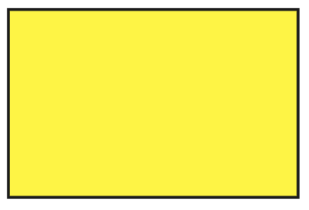
\includegraphics[width=0.78681in,height=0.53472in]{img/IMFmanual-img020.png}  &
    {\centering Product Block}

    \centering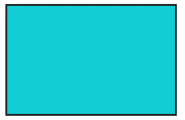
\includegraphics[width=0.84297in,height=0.54686in]{img/IMFmanual-img021.png}  &
    {\centering Location Block}

    \centering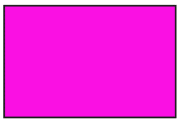
\includegraphics[width=0.8326in,height=0.55237in]{img/IMFmanual-img022.png}  &
    {\centering Installed Block}

    \centering\arraybslash  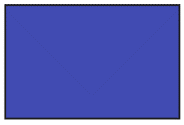
\includegraphics[width=0.83927in,height=0.56774in]{img/IMFmanual-img023.png}
    \\\hline
    &
    \centering{\bfseries Aspect Terminal} &
    {\centering Function Terminal}

    \centering
\includegraphics[width=0.35063in,height=0.33245in]{img/IMFmanual-img024.png}  &
    {\centering Product Terminal}

    \centering
\includegraphics[width=0.33351in,height=0.33351in]{img/IMFmanual-img025.png}  &
    {\centering Location Terminal}

    \centering Not used &
    {\centering Installed Terminal}

    \centering\arraybslash  
\includegraphics[width=0.34253in,height=0.3131in]{img/IMFmanual-img026.png} \\\hline
    \multicolumn{2}{|m{1.11286in}|}{\centering \textbf{Aspect Object}} &
    {\centering Function Object}

    \centering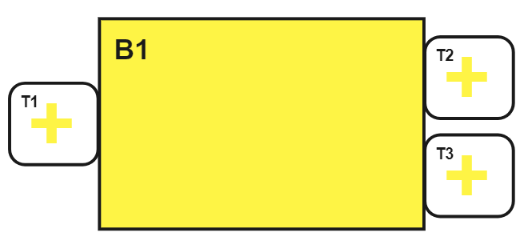
\includegraphics[width=1.27224in,height=0.59884in]{img/IMFmanual-img027.png}  &
    {\centering Product Object}

    \centering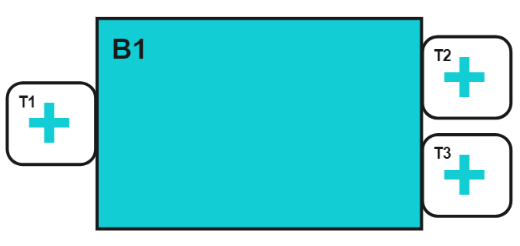
\includegraphics[width=1.25119in,height=0.59191in]{img/IMFmanual-img028.png}  &
    {\centering Location Object}

    \centering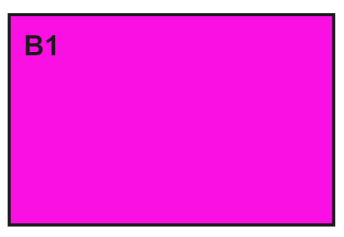
\includegraphics[width=0.81215in,height=0.55953in]{img/IMFmanual-img029.png}  &
    {\centering Installed Object}

    \centering\arraybslash  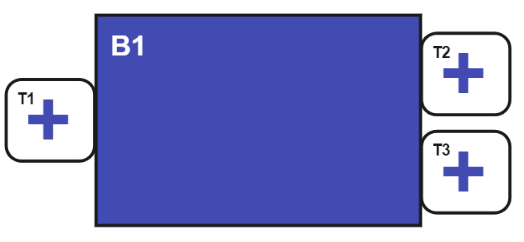
\includegraphics[width=1.21847in,height=0.56273in]{img/IMFmanual-img030.png}
    \\\hline
  \end{supertabular}
\end{table}

\section{Objectives}
The IMF language is designed to conform to the relevant objectives given in \autoref{ch:Section 1.2}:

\begin{itemize}
  \item \emph{The language shall be made so that the SMEs themselves are users of the framework.} This means that the
        IMF language must:

        \begin{itemize}
          \item Contain a limited set of elements (vocabulary) and grammar rules such that it is easy to learn and simple to
                use.
        \end{itemize}
  \item \emph{The language shall provide incremental value}. This means that the IMF language must be:

        \begin{itemize}
          \item Designed such that one can have an incremental approach and model fragment by fragment.
        \end{itemize}
  \item \emph{The language shall be scalable across disciplines, work processes, and the value chain}. This means that
        the IMF language must:

        \begin{itemize}
          \item Enable SMEs from a range of disciplines to fully express their design using the same modelling principles.
          \item Enable the SMEs to express different levels of precision as part of iterations of their design.
          \item Enable use in different phases of a project (concept, detail engineering, manufacturing, etc.).
        \end{itemize}
  \item \emph{The language shall have the precision of machine interpretation to allow automated verification}. This
        means that the IMF language must:

        \begin{itemize}
          \item Be precise and unambiguous.
          \item Allow translation into an ontology language that can use automated reasoning techniques in combination with
                information in the RDL for verification.
        \end{itemize}
\end{itemize}
\section{The IMF Language}
This section formally defines the IMF language. The language is introduced in subsections
that contain an introduction, a set of formal definitions and a visualization guide.

The formal definitions are accompanied by a structural specification diagram. The diagrams are UML class diagrams and are drawn using the following constructs:

\begin{itemize}
  \item Classes, marked with the icon ``C''. Classes may have
        ``fields'' that can hold values, fields are not used to represent relationships.
  \item Abstract classes, marked with an icon ``A'', are classes that are not intended to be
        instantiated.
  \item Enumerations, marked with the icon ``E'', are used to represent UML classes with a
        limited list of instantiations and where the instantiations are defined in the IMF language.
  \item Stereotypes, marked with an icon ``S'' are used to represent a class structure that is
        not intended to be explicitly represented in the language, but represents a tag and a convenient repetitive
        structure. Classes that use stereotypes indicate this with {\textless}{\textless} stereotype
          {\textgreater}{\textgreater} above the class name.
  \item Subclass relationships between classes, which are drawn using directed relations with an open arrow.
  \item Directed associations (relations) between classes, which are marked with a name and possibly a cardinality. If
        no cardinality is given, then the cardinality is 0--many.
  \item Composition relations, drawn with a filled diamond as arrow, indicates a strong dependency to the target of the
        relationship; the target is considered as a part of the source and cannot exist independently of the source of the
        relationship.
  \item Aggregation relations, drawn with an open diamond as arrow, indicates a weak dependency to the target of the
        relationship than to that of a composition relation, the target is considered as part of the source but can exist
        independently of the source of the relationship.
\end{itemize}
\autoref{fig:Figure 12} illustrates many of the constructs used.

\begin{figure}[htb]
  \centering
  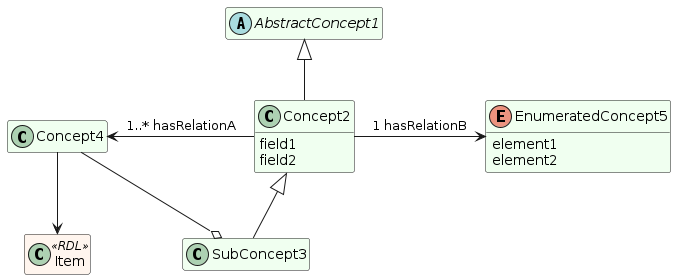
\includegraphics[width=5in,height=2.0625in]{img/IMFmanual-img031.png}
  \caption{Diagram exemplifying different UML class diagram constructs}
  \label{fig:Figure 12}
\end{figure}

\subsection{Preliminaries}
The language consists of \emph{objects}, \emph{relations}, and \emph{attributes}. A relation is a set of \emph{relationships}, where a relationship is a connection between two objects.  Only objects
may have attributes. To assign attributes to a relationship, an object that represents the relationship must be
created (this is sometimes called reification); we call such objects \emph{association points}.

\subsection{Model}
The objects in the IMF language are called \emph{Elements. }Elements are organized in
\emph{Models}. Most of the objects in the IMF language are Identified, which means that that they have an identifier and a set of common metadata and provenance data. \autoref{fig:Figure 13} illustrates
these constructs.

\begin{figure}[htb]
  \centering
  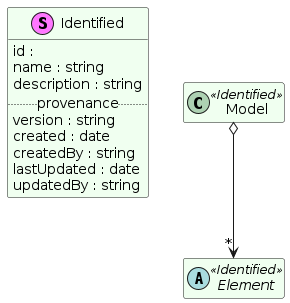
\includegraphics[width=3.02083in,height=3.15625in]{img/IMFmanual-img032.png}
  \caption{Model and Identified}
  \label{fig:Figure 13}
\end{figure}

\subsection{Elements}
We distinguish between two different kinds of Elements: \emph{Blocks} and
\emph{Terminals}.

A Block is the basic building block of the IMF language. A Block represents something of interest to the SME by
setting the boundaries of anything which is convenient to treat as an entity. This could be a whole industry plant, a
pump system, or a small location of interest.

A Terminal represents a channel of communication (of any type to media, such as information, material, energy) for a
Block; hence a Terminal cannot exist without a Block. A Block may have any number of Terminals that each represent a different communication channel or port with which the
Block may receive input and/or give output. A Terminal that is specified to only receive input is called an
\emph{InputTerminal}. A Terminal that is specified to only give output is called an \emph{OutputTerminal}. A
Terminal that is neither specified as an InputTerminal nor OutputTerminal (and is simply called a Terminal), may both
receive input and give output. See \autoref{fig:Figure 14} for a diagram of these constructs. \autoref{fig:Figure 17} displays the same diagram,
with association points and reified relations included.

\subsubsection{Formal definitions}


\begin{figure}[htb]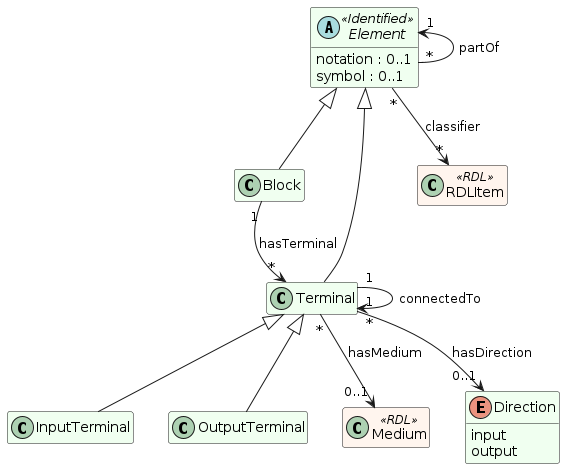
\includegraphics[width=5.48958in,height=4.55178in]{img/IMFmanual-img033.png}
  \caption{Core Elements}
  \label{fig:Figure 14}
\end{figure}

\textit{An Element is an object with a collection of attributes. }

\textit{A Block is an Element that is used to describe an entity}\footnote{{An entity is a thing with distinct
      and independent existence.}\par }\textit{.}

{\itshape
  A Terminal is an Element that is used to describe the input or output of a Block, and hence its boundaries. A Terminal
  is associated with exactly one Block. A Block may have any number of Terminals. }

{\itshape
  hasTerminal is the relation that connects a Block to a Terminal, i.e., the domain and range of the relation is
  respectively Block and Terminal. The relation is inverse functional since a Terminal can only be associated to one
  Block.}

{\itshape
  Block and Terminal are disjoint; nothing is both a Block and a Terminal.}

\textit{An InputTerminal is a Terminal that describes only the input of a Block. }

\textit{An OutputTerminal is a Terminal that describes only the output of a Block.}

{\itshape
  InputTerminal and OutputTerminal are disjoint; nothing is both an InputTerminal and an OutputTerminal.}

\subsubsection{Visualization}
A Block is visualized as a rectangular box, see \autoref{fig:Figure 15}.

\begin{figure}[htb]
  \centering
  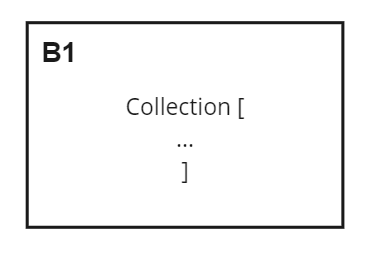
\includegraphics[width=1.82456in,height=1.23878in]{img/ontology/element-block.png}
  \caption{A Block.}
  \label{fig:Figure 15}
\end{figure}

A Terminal is visualized as a small box with a plus (+) sign, as shown in \autoref{fig:Figure 16}.

\begin{figure}[htb]
  \centering
  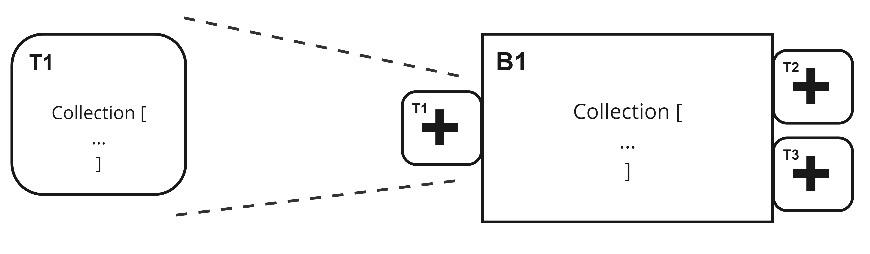
\includegraphics[width=3.94162in,height=1.15217in]{img/ontology/element-terminal.jpg}
  \caption{A Terminal.}
  \label{fig:Figure 16}
\end{figure}

\subsection{Breakdowns and Topology: partOf and connectedTo}
Central to the IMF describing objects at different levels of abstraction and generality.
Abstract, high-level descriptions may recursively be broken down into more detailed, fine-grained descriptions. All
objects may be broken down into more detailed objects, as long as the objects are of the same type, and so that any
object is the result of the breakdown of one object only; that is, the breakdown structure must form a tree where
every object in the tree may have many children but can only have a single parent. In IMF, the partOf relation is
used for modelling breakdown structures. If the relationship partOf(A,B) is true, we may informally express this as
that ``A is part of B'' or ``B has A as part''.

Topology, how objects are connected, is modelled using the connectedTo relation. This relation connects two Terminals
of two Blocks. A Terminal may have a direction and a specified media, and the intuition is that the directions and media of the
connected Terminals must match, e.g., an OutputTerminal must be connected to an InputTerminal, and a Terminal that
outputs water cannot be connected to a Terminal that takes electricity as input, \emph{however this constraint is
  not enforced by the formal language specification}.

In contrast to an object, a relation cannot not hold a collection of attributes. To assign attributes to a relationship, the relationship must be associated with an object called
association point. The association point of a connectedTo relationship is called \emph{ConnectionPoint}. The
association point for a partOf relationship is called a \emph{BreakdownPoint}.

\subsubsection{Formal definitions}
\begin{figure}[htb]
  \centering
  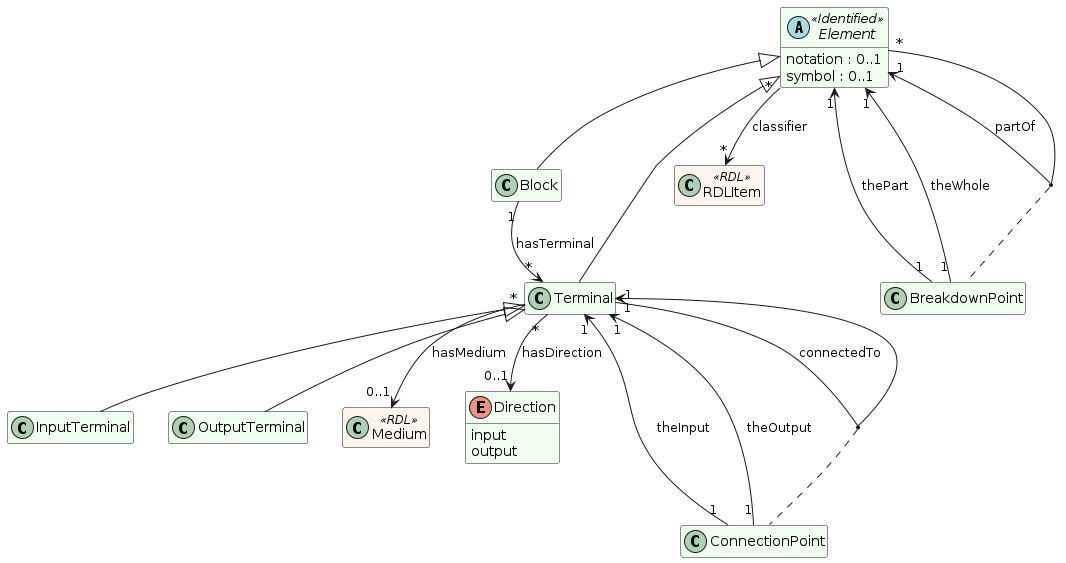
\includegraphics[width=6.45834in,height=3.41753in]{img/IMFmanual-img036.png}
  \caption{Core Elements with reified relationships/association points}
  \label{fig:Figure 17}
\end{figure}

{\itshape
partOf is a relation between Elements; the domain and range of the relation is Element. However, partOf may only
relate Elements of the same type, i.e., a Block may only have Blocks as parts, and a Terminal may only have Terminals
as parts.}

{\itshape
partOf is functional; an Element may only be part of at most one Element.}

{\itshape
partOf is irreflexive; an Element may not be part of itself.}

{\itshape
The inverse relation of partOf is hasPart.}

\textit{{A partOf relationship may be reified, the reification object
      is called a BreakdownPoint. A BreakdownPoint is an Element that describes a partOf relationship. }}

{\itshape
  connectedTo is a relation between Terminals.  }

{\itshape
  connectedTo is functional and inverse functional; a Terminal is connected to at most one Terminal.}

{\itshape
  connectedTo is irreflexive; a Terminal may not be connected to itself.}

{\itshape
  A connectedTo relationship may be reified, the reification object is called a ConnectionPoint. A ConnectionPoint is an
  Element that describes a connectedTo relationship.}

\autoref{tab:Table 4}\textit{{ gives an overview of the partOf and connectedTo
      relations.}}

\begin{table}[htb]
  \centering
  \caption{Summary of partOf and connectedTo relations.}\label{tab:Table 4}
  \begin{supertabular}{|m{1.2962599in}|m{1.7913599in}|m{1.6934599in}|m{1.3968599in}|}
    \hline
    {\bfseries Relation} &
    {\bfseries Domain} &
    {\bfseries Range} &
    {\bfseries Cardinality}\\\hline
    { partOf} &
    { Block/Terminal} &
    { Block/Terminal} &
    { Many -- 1}\\\hline
    {connectedTo} &
    { Terminal} &
    { Terminal} &
    { 1 - 1}\\\hline
  \end{supertabular}
\end{table}

\subsubsection{Visualization}
A partOf relationship partOf(B2, B1) is illustrated with an arrow pointing from the top of B2 to the bottom of B1, see \autoref{fig:Figure 18}.

\begin{figure}[htb]
  \centering
  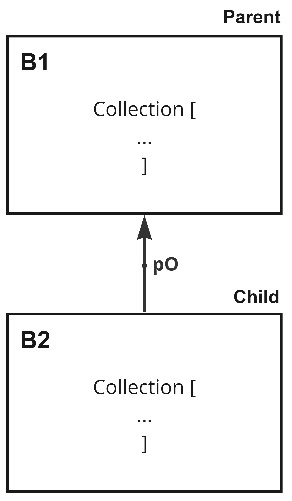
\includegraphics[width=1.3221in,height=2.26735in]{img/ontology/element-partOf.jpg}
  \caption{A partOf relationship between Blocks }
  \label{fig:Figure 18}
\end{figure}

A connectedTo relationship can be illustrated in two ways. A connectedTo relationship with no
associated ConnectionPoint is visualized as line between the Terminals it connects. A connectedTo relationship with
an associated ConnectionPoint is visualized by representing the ConnectionPoint as a split circle placed in the
middle of the line between the connected Terminals. See \autoref{fig:Figure 19}.

\begin{figure}[htb]
  \centering
  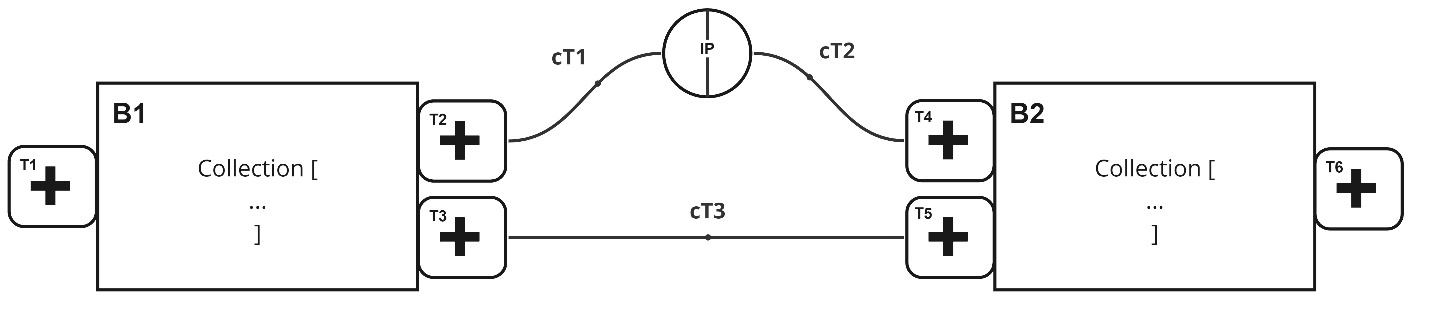
\includegraphics[width=6.5in,height=1.425in]{img/ontology/element-connectedTo.jpg}
  \caption{Two connectedTo relationships}
  \label{fig:Figure 19}
\end{figure}

\subsection{Attributes}
Associated with an Element is an arbitrary number of attributes, here called attribute
values. Attribute values may be grouped together into attribute groups that typically contain related attributes. An
attribute group may have a name and description that explain the intended use of the attributes.

\subsubsection{Formal definitions}
\begin{figure}[htb]
  \centering
  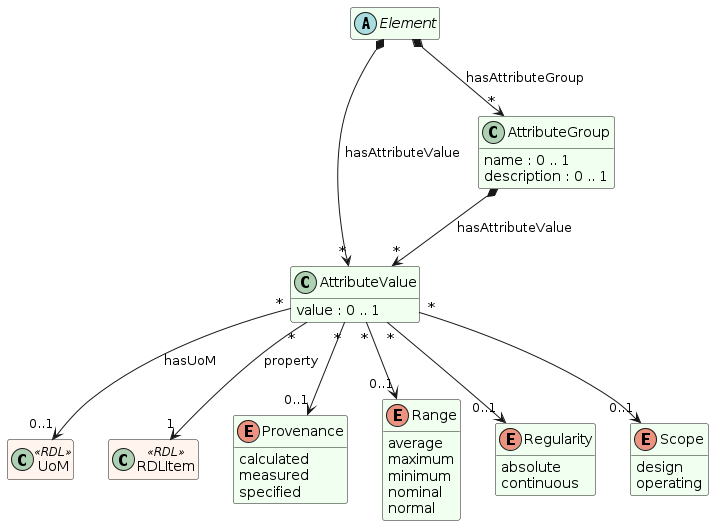
\includegraphics[width=5in,height=3.6875in]{img/IMFmanual-img039.png}
  \caption{Element's AttributeValues}
  \label{fig:Figure 20}
\end{figure}

The attributes of an Element, called AttributeValues, are related to the Element is belongs to via a hasAttributeValue
relationship. An AttributeValue must state a property, which is taken from a reference data library, and may state a
unit of measure (UoM), also taken from a reference data library. Additionally, the AttributeValue may be qualified
with a Provenance, Range, Regularity and Scope qualifier. See \autoref{fig:Figure 20}.

\subsection{Aspects}
The concept of aspects is taken from ISO/IEC 81346-1~\cite{81346-1}. Aspects allow us to view a
facility asset from different perspectives and give a structuring mechanism for separating different types of
information about an object, and hence allows scalability across disciplines, work processes, and the value chain.

Aspects act like filters on a facility asset and highlight the information that is of relevance~\cite{81346-1}. The IMF language
defines four elementary aspects, these are given in \autoref{tab:Table 5}. AspectElements, which are Elements with exactly one
Aspect, represent a distinct view on an entity and which can be related across aspects, see \autoref{fig:Figure 21}. Note that it is possible to introduce more aspects to support other ways of viewing a Facility Asset.

We strictly separate between two types of relations; intra-aspect relations are relations that may only relate
AspectElements of the same Aspect, while inter-aspect relations may only relate AspectElement of different Aspects.

The inter-aspect relations are asProduct, asFunction, asLocation, and asInstalled, see \autoref{fig:Figure 22}. These relations
always relate Elements of the same kind, a Block must be related to a Block, and a Terminal must be related to a
Terminal. The range of these relations are as indicated by the name of the relation, e.g., the range of asProduct is
an AspectElement of the ProductAspect. The relations may have different cardinality constraints depending on the
domain of the relation. The intuition for these relations is that they relate an AspectElement to a different
AspectElement that represents a different perspective on the same entity.

\subsubsection{Formal definitions}
\begin{figure}[htb]
  \centering
  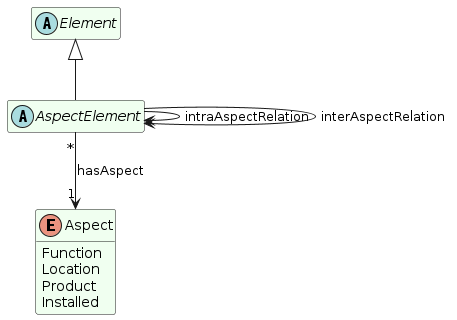
\includegraphics[width=4.50752in,height=3.15625in]{img/IMFmanual-img040.png}
  \caption{AspectElement and Aspects}
  \label{fig:Figure 21}
\end{figure}

\textit{An Aspect is a particular way of viewing an object. There are at least four different Aspects, these are
  listed in }\autoref{tab:Table 4}\textit{. }

\begin{table}[htb]\centering\caption{Definition of different aspects and their associated
    prefix and colors.}\label{tab:Table 5}
  \begin{supertabular}{|m{1.6899599in}|m{3.16986in}|m{0.5343598in}|m{0.78375983in}|}
    \hline
    {\bfseries Aspect} &
    {\bfseries Definition} &
    {\bfseries Prefix} &
    {\bfseries Color}\\\hline
    {\bfseries The Function Aspect (F)} &
    \textit{The Function Aspect is about the requirements to the intended activity.} &
    \centering = &
    Yellow\\\hline
    {\bfseries The Product Aspect (P)} &
    \textit{The Product Aspect is about the specification of the artifact.} &
    \centering - &
    Cyan\\\hline
    {\bfseries The Location Aspect (L)} &
    \textit{The Location Aspect is about the specification of the spatial extension of the artifact.} &
    \centering + &
    Magenta\\\hline
    {\bfseries The Installed Aspect (I)} &
    \textit{The Installed Aspect is about the documentation of the actual }\textit{artifact.} &
    \centering :: &
    { Dark Blue}\\\hline
  \end{supertabular}
\end{table}

{\itshape
An AspectElement is an Element with exactly one Aspect. The relation between an AspectElement and its Aspect is
hasAspect. hasAspect is functional. }

\textit{For convenience, we introduce names for each AspectElement of a specific type and with a given Aspect, these
  are listed in }\autoref{tab:Table 6}\textit{.}

\begin{table}[htb]\centering\caption{Different Aspect Elements.}\label{tab:Table 6}
  \begin{supertabular}{|m{1.1975598in}|m{1.2996598in}|m{1.2996598in}|m{1.4962599in}|}
    \hline
    {\bfseries Elements /}

    {\bfseries Aspects} &
    {\bfseries Element} &
    {\bfseries Block (B)} &
    {\bfseries Terminal (T)}\\\hline
    {\bfseries Function (F)} &
    Function Element &
    Function Block (\textbf{FB}) &
    Function Terminal (\textbf{FT})\\\hline
    {\bfseries Product (P)} &
    Product Element &
    Product Block (\textbf{PB}) &
    Product Terminal (\textbf{PT})\\\hline
    {\bfseries Location (L)} &
    { Location Element} &
    {Location Block (}\textbf{{LB}}{)} &
    {Location Terminal (}\textbf{{LT}}{)}\\\hline
    {\bfseries Installed (I)} &
    { Installed Element} &
    {Installed Block (}\textbf{{IB}}{)} &
    {Installed Terminal (}\textbf{{IT}}{)}\\\hline
  \end{supertabular}
\end{table}

{\itshape
An intraAspectRelation is a relation between AspectElements of the same Aspect. An interAspectRelation is a relation
between AspectElements of different Aspects.}

{\itshape
When restricted to AspectElements, the following relations are intraAspectRelations: hasTerminal, hasPart,
connectedTo.}

{\itshape
An interAspectRelation relationship either relates two Blocks, or two Terminals. It may not relate a Block to a
Terminal, or a Terminal to a Block.}

\begin{figure}[htb]
  \centering
  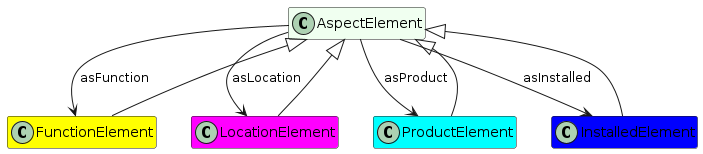
\includegraphics[width=6.44424in,height=1.40968in]{img/IMFmanual-img041.png}
  \caption{Inter-aspect relations}
  \label{fig:Figure 22}
\end{figure}

{\itshape
The following relations are interAspectRelations: asProduct, asFunction, asLocation, asInstalled.}

{\itshape
asProduct is an interAspectRelation from FunctionElements and InstalledElements to ProductElements. A FunctionElement
may be related to zero to many ProductElements via the hasProduct relation. An InstalledElement may only be related
to at most one ProductElement via the hasProduct relation.}

{\itshape
asFunction is an interAspectRelation from ProductElements to FunctionElements. A ProductElement may be related to zero
to many FunctionElements via the asFunction relation.}

{\itshape
asLocation is an interAspectRelation from ProductElements to LocationElements. A ProductElement may be related to at
most one LocationElement.}

{\itshape
asInstalled is an interAspectRelation from ProductElements to InstalledElements. A ProductElement may be related to
zero to many InstalledElements. }

\autoref{tab:Table 7} gives an overview of all interAspectRelations with their domain and range and cardinality.

\begin{table}[htb]\centering\caption{Inter-aspect relations and their domain and range and
    cardinality}\label{tab:Table 7}
  \begin{supertabular}{|m{1.5906599in}|m{1.7621598in}|m{2.0607598in}|m{0.7642598in}|}
    \hline
    {\bfseries\itshape Relation} &
    {\bfseries\itshape Domain} &
    {\bfseries\itshape Range} &
    {\bfseries\itshape Cardinality}\\\hline
    \textit{{asProduct}} &
    {\itshape FunctionElement} &
    {\itshape ProductElement} &
    {\itshape 1 - many}\\\hline
    {\itshape asProduct} &
    {\itshape InstalledElement} &
    {\itshape ProductElement} &
    {\itshape 1 - 1}\\\hline
    \textit{{asFunction}} &
    {\itshape ProductElement} &
    {\itshape FunctionElement} &
    {\itshape 1 -- many}\\\hline
    \textit{{asLocation}} &
    {\itshape ProductElement} &
    {\itshape LocationElement} &
    \textit{{1 -- 1}}\\\hline
    {\itshape asInstalled} &
    {\itshape ProductElement} &
    {\itshape InstalledElement} &
    {\itshape 1 -- many}\\\hline
  \end{supertabular}
\end{table}

\subsubsection{Visualization}
Each aspect is given a distinct color, as listed in \autoref{tab:Table 8}. AspectElements are visualized by using this color to fill
the shape of the Element. Relationships are drawn without color.

\subsubsection{Intuitions}
The intended intuition and visualization for every AspectElements is summarized in \autoref{tab:Table 8} and \autoref{tab:Table 9}.

\begin{figure}[htb]
  \centering
  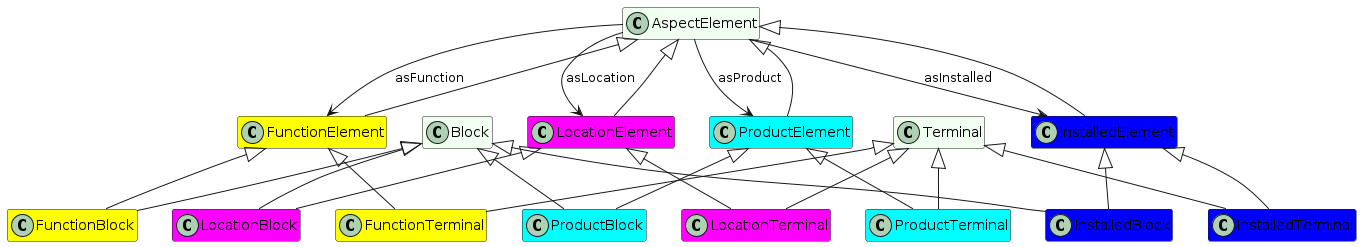
\includegraphics[width=6.46875in,height=1.17246in]{img/IMFmanual-img042.png}
  \caption{AspectElements and convenience constructs}
  \label{fig:Figure 23}
\end{figure}

\begin{table}[htb]\centering\caption{Aspect Blocks and their intuition.}\label{tab:Table 8}
  \begin{supertabular}{|m{1.2996598in}|m{3.75666in}|m{1.2121599in}|}
    \hline
    {\bfseries Name} &
    {\bfseries Intuition} &
    {\bfseries Graphics}\\\hline
    Function Block (\textbf{FB)} &
    A function block holds the requirements to intended activity. &
    \centering\arraybslash  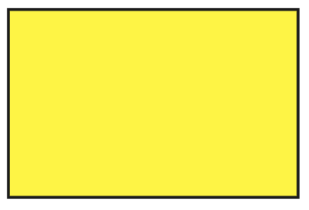
\includegraphics[width=0.87059in,height=0.59167in]{img/IMFmanual-img020.png}
    \\\hline
    Product Block (P\textbf{B)} &
    A product block holds the specification of an artifact. &
    \centering\arraybslash  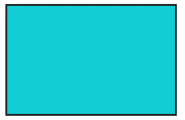
\includegraphics[width=0.84297in,height=0.54686in]{img/IMFmanual-img021.png}
    \\\hline
    Location Block (\textbf{LB)} &
    A location block holds the specification to the spatial extension of an artifact and requirements imposed by its
    spatial position in the Location Breakdown. &
    \centering\arraybslash  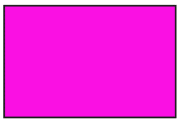
\includegraphics[width=0.8326in,height=0.55237in]{img/IMFmanual-img022.png} \\\hline
    Installed Block (\textbf{IB)} &
    An installed block holds the documentation of an installed artifact.  &
    \centering\arraybslash  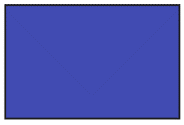
\includegraphics[width=0.83927in,height=0.56774in]{img/IMFmanual-img023.png}
    \\\hline
  \end{supertabular}
\end{table}

\begin{table}[htb]\centering\caption{Aspect Terminals and their intuition.}\label{tab:Table 9}
  \begin{supertabular}{|m{1.3948599in}|m{3.9566598in}|m{0.8191598in}|}
    \hline
    {\bfseries Name} &
    {\bfseries Intuition} &
    {\bfseries Graphics}\\\hline
    Function Terminal (\textbf{FT}) &
    Requirements to one input/output stream state of a purpose activity &
    \centering\arraybslash  
\includegraphics[width=0.35063in,height=0.33245in]{img/IMFmanual-img024.png}
    \\\hline
    Product Terminal (\textbf{PT}) &
    Specification of one input/output/bidirectional terminal of an artifact &
    \centering\arraybslash  
\includegraphics[width=0.33351in,height=0.33351in]{img/IMFmanual-img025.png}
    \\\hline
    Location Terminal (\textbf{LT}) &
    \centering Not used &
    \centering\arraybslash Not used\\\hline
    Installed Terminal (\textbf{IT}) &
    Documentation of an installed artifact terminal. &
    \centering\arraybslash  
\includegraphics[width=0.34253in,height=0.3131in]{img/IMFmanual-img026.png} \\\hline
  \end{supertabular}
\end{table}

\autoref{tab:Table 10} to \autoref{tab:Table 13} give overview of the different relations between Aspect Elements and their intuitions.

\begin{table}[htb]\centering\caption{partOf relations and their intuition.}\label{tab:Table 10}
  \begin{supertabular}{|m{1.1975598in}|m{4.94136in}|}
    \hline
    {\bfseries partOf relation} &
    {\bfseries Intuition}\\\hline
    partOf(\textbf{FB1},\textbf{FB2}) &
    The purpose activity of Function Block \textbf{FB1} is a sub-activity of that of Function Block \textbf{FB2}\\\hline
    partOf(\textbf{PB1},\textbf{PB2}) &
    The artifact of Product Block \textbf{PB1} is a sub-assembly of the artifact of Product Block \textbf{PB2}\\\hline
    partOf(\textbf{LB1},\textbf{LB2}) &
    The location of Location Block \textbf{LB1} is located in the location of Location Block \textbf{LB2}\\\hline
    partOf(\textbf{IB1},\textbf{IB2}) &
    The artifact of Installed Block \textbf{IB1} is sub-assembly of the artifact of Installed Block \textbf{IB2}\\\hline
  \end{supertabular}
\end{table}

\begin{table}[htb]\centering\caption{hasTerminal relations and their intuition.}\label{tab:Table 11}
  \begin{supertabular}{|m{1.1975598in}|m{0.90595984in}|m{4.00386in}|}
    \hline
    \textbf{hasTerminal relation} &
    {\bfseries Specification of} &
    {\bfseries Intuition}\\\hline
    hasTerminal(\textbf{FB},\textbf{FT}) &
    Activity &
    The media state of Function Terminal \textbf{FT} is the input/output of the purpose activity in Function Block\textbf{
      FB}\\\hline
    hasTerminal(\textbf{PB},\textbf{PT}) &
    Artifact &
    The Product Terminal \textbf{PT} is a specification of one input/output terminal of the artifact of Product Block
    \textbf{PB}\\\hline
    hasTerminal(\textbf{LB},\textbf{LT}) &
    Location &
    Not used\\\hline
    hasTerminal(\textbf{IB},\textbf{IT}) &
    Artifact &
    The installed terminal \textbf{IT} holds documentation of an installed artifact terminal \textbf{IB}\\\hline
  \end{supertabular}
\end{table}


\begin{table}[htb]\centering\caption{connectedTo relations and their intuition.}\label{tab:Table 12}
  \begin{supertabular}{|m{1.2962599in}|m{1.0038599in}|m{3.80596in}|}
    \hline
    \textbf{connectedTo Relation} &
    {\bfseries Specification of} &
    {\bfseries Intuition}\\\hline
    connectedTo(\textbf{FT1},\textbf{FT2}) &
    Activity &
    The media state of Function Terminal \textbf{FT1} is equal to that of Function Terminal \textbf{FT2}.\\\hline
    connectedTo(\textbf{PT1},\textbf{PT2})

    &
    Artifact &
    The stream of Product Terminal \textbf{PT1} is physically connected to the steam of Product Terminal \textbf{PT}

    \\\hline
    connectedTo(\textbf{LT1},\textbf{LT2})

    &
    Location &
    Not used

    \\\hline
    connectedTo(\textbf{IT1},\textbf{IT2})

    &
    Artifact &
    The stream of Installed Terminal \textbf{IT1} is physically connected to the stream of Installed Terminal
    \textbf{IT2}.\\\hline
  \end{supertabular}
\end{table}

\begin{table}[htb]\centering\caption{inter-aspect relations and their intuition.}\label{tab:Table 13}
  \begin{supertabular}{|m{1.2962599in}|m{4.85036in}|}
    \hline
    {\bfseries Inter-Aspect Relation} &
    {\bfseries Intuition}\\\hline
    asProduct(\textbf{FB},\textbf{PB}) &
    The artifact of Product Block\textbf{ PB} realizes the entire or parts of the purpose of Function Block\textbf{
      FB}\\\hline
    asProduct(\textbf{FT},\textbf{PT}) &
    Artifact Terminal of Product Terminal \textbf{PT} provides physical connection of the media state of Function Terminal
    \textbf{FT}\\\hline
    asLocation(\textbf{PB},\textbf{LB}) &
    The Location Block \textbf{LB }describes the spatial extension of the artifact of Product Block \textbf{PB}\\\hline
    asInstalled(\textbf{PB},\textbf{IB}) &
    The installed artifact of Installed Block \textbf{IB} realizes the artifact specifications of Product Block
    \textbf{PB}\\\hline
    asInstalled(\textbf{PT},\textbf{IT}) &
    The installed artifact terminal Installed Terminal \textbf{IT} realizes the terminal specifications of Product
    Terminal \textbf{PT}\\\hline
  \end{supertabular}
\end{table}

\section{The Aspect Object}
For convenience we introduce the term AspectObject to designate an AspectElement Block
with all its Terminals.

Definition: \textbf{The Aspect Object -- }\textit{An Aspect Object is a composite object structure comprised of an
  Aspect Block}\textbf{\textit{ }}\textit{and all its Aspect Terminals that are connected through hasTerminal
  relationships. An Aspect Object has a single Aspect, which is the same as the Aspect of the Block and its Terminals.
}

\begin{figure}[htb]
  \centering
  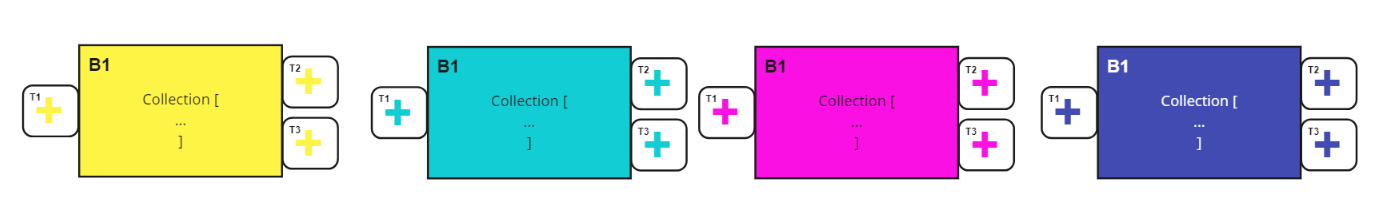
\includegraphics[width=6.5in,height=1.04931in]{img/IMFmanual-img043.png}
  \caption{Four different Aspect Objects: Function, Product, Location, and Installed.}
  \label{fig:Figure 24}
\end{figure}

The Aspect Object makes the SME able to talk about the Facility Asset itself (the Block) and its boundaries (the
Terminals) in a precise and effective way. Given the aspects defined in \autoref{tab:Table 5}, we have four different Aspect
Objects, as shown in \autoref{fig:Figure 24}. We use the colors (and prefixes) given in \autoref{tab:Table 5} to illustrate which aspect each one
resides in.

For convenience, when we refer to an Aspect Object of a certain aspect, we replace the word `Aspect' for the given
aspect the Aspect Object belongs to. For example, we say `Function Object' instead of the general designation `Aspect
Object'.

In the following sections and chapters, we will primarily use the Aspect Object to create IMF models (\autoref{ch:Chapter 5}) and
IMF Types (\autoref{ch:Chapter 6}).

\section{Intuitions on partOf Breakdowns}
\label{ch:Section 4.4}
It is important for SMEs to express various levels of precision in
their design. The partOf relation is a mechanism for this. \autoref{fig:Figure 25} shows three Aspect Blocks (\textbf{AB1},
\textbf{AB2}, and \textbf{AB3}) and two partOf relations (\textbf{pO1} and \textbf{pO2}). Together they form a
\emph{Breakdown}, also referred to as a \emph{Hierarchy}. We use a grey color on the aspect-independent Aspect
Objects.

The partOf relation promotes a \emph{System-Of-Systems} way of thinking. Using the Breakdown to the left in Figure
25 as an example, we can think of \textbf{AB2} and \textbf{AB3} as two independent systems in context as part of a
larger, more complex system \textbf{AB1}. The system-of-system approach facilitates a recursive way to create deeper
Breakdowns to connect several levels of the design shown to the right in \autoref{fig:Figure 25}.

Breakdowns can be interpreted in different ways. From a top-down view, it is reasonable to think about the Breakdown
formed by the partOf relation as a mechanism for decomposing systems into sub-systems. Thus, in the Breakdown in
\autoref{fig:Figure 25}, \textbf{AB2} and \textbf{AB3} can be viewed as sub-components of \textbf{AB1}.

\begin{figure}[htb]
  \centering
  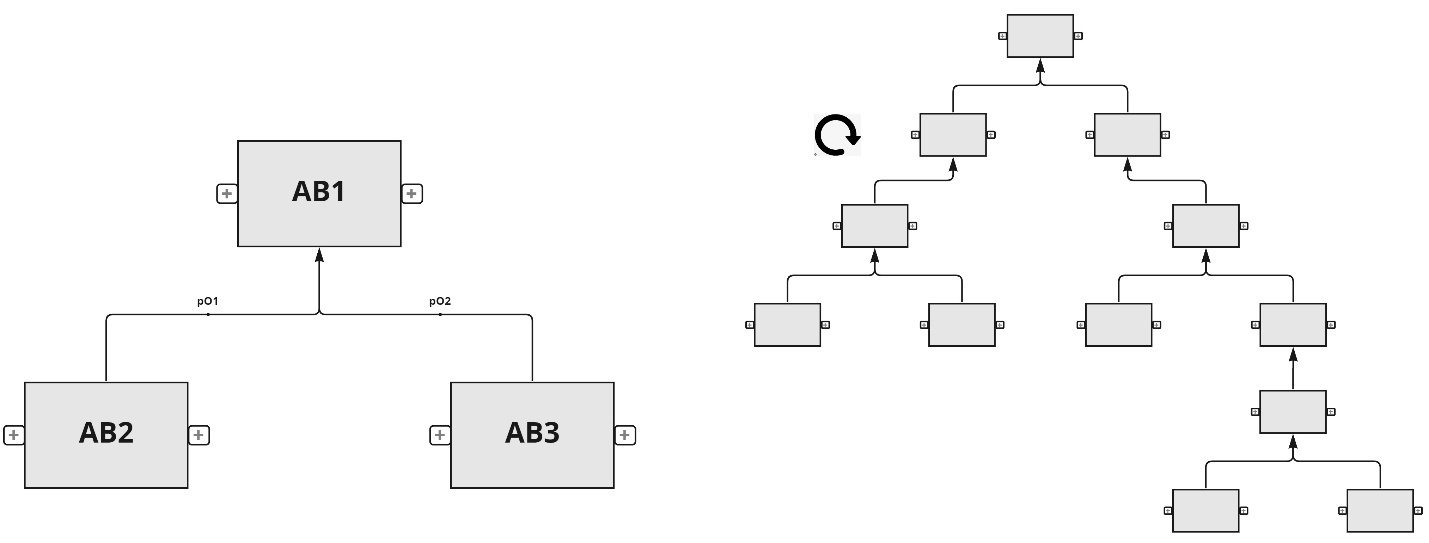
\includegraphics[width=1\textwidth]{img/IMFmanual-img044.jpg}
  \caption{A small breakdown with a parent AB1 and two children, AB2 anf AB3 to the left. A deeper Breakdown to the right.}
  \label{fig:Figure 25}
\end{figure}

From a bottom-up view, it is reasonable to think about the Breakdown as a grouping and abstraction mechanism. Again,
using the Breakdown to the left in \autoref{fig:Figure 25} we can say that \textbf{AB2 }and \textbf{AB3 }are part of the grouping
or abstraction formed by \textbf{AB1}. Furthermore, this is useful when it is convenient to treat a complex system
(\textbf{AB1}) as a `black box' by hiding details (\textbf{AB2 }and\textbf{ AB3}) and postponing dealing with them to
a later stage. Top-down and Bottom-up approaches to modeling is further discussed in \autoref{ch:Chapter 5.4}

Breakdowns can be created in all aspects. The intuition about what they represent is given in \autoref{tab:Table 14}.

\begin{table}[htb]\centering\caption{Aspect Breakdowns and their interpretation.}\label{tab:Table 14}
  \begin{supertabular}{|m{1.2962599in}|m{4.06286in}|m{0.8073598in}|}
    \hline
    {\bfseries Aspect Breakdown} &
    \textbf{Intuition} &
    {\bfseries Color}\\\hline
    {\bfseries Function Aspect Breakdown} &
    \textit{The Function Aspect Breakdown specifies a breakdown of activities into sub-activities.} &
    Yellow\\\hline
    {\bfseries Product Aspect Breakdown} &
    {\itshape The Product Aspect Breakdown specifies an assembly breakdown of artifacts.} &
    Cyan\\\hline
    {\bfseries Location Aspect Breakdown} &
    {\itshape The Location Aspect Breakdown specifies a spatial breakdown.} &
    Magenta\\\hline
    {\bfseries Installed Aspect Breakdown} &
    {\itshape The Installed Aspect Breakdown documents the actual assembly breakdown of artifacts. }
    &
    { Dark Blue}\\\hline
  \end{supertabular}
\end{table}

\section{Intuitions on connectedTo Topologies}
\label{ch:Section 4.5}
SMEs must be able to express how Facility Assets are connected to
one another. Another way to think about it is the need to express what type of media (e.g., Material, Energy, Force,
or Information) is streaming between the Facility Assets. \autoref{fig:Figure 26} shows three Aspects Blocks (\textbf{AB1},
\textbf{AB2}, and \textbf{AB3}), two Interface Points, and a set of connectedTo relationships. Connected they form a
\emph{Topology}. We use a grey color on the aspect-independent Aspect Objects.

The connectedTo relation promotes a \emph{System-to-System} way of thinking. Using the \emph{Topology} in Figure
26 as an example we can think that some type of media is streaming from \textbf{AB1}, through \textbf{AB2}, and
further on to \textbf{AB3}. The system-to-system approach facilitates a way to create large and complex interactions
between Facility Assets through feedforward and feedback loops etc., as shown in \autoref{fig:Figure 27}. Modelling topologies of
different Facility Assets are further discussed in \autoref{ch:Chapter 5.4}.

\begin{figure}[htb]
  \centering
  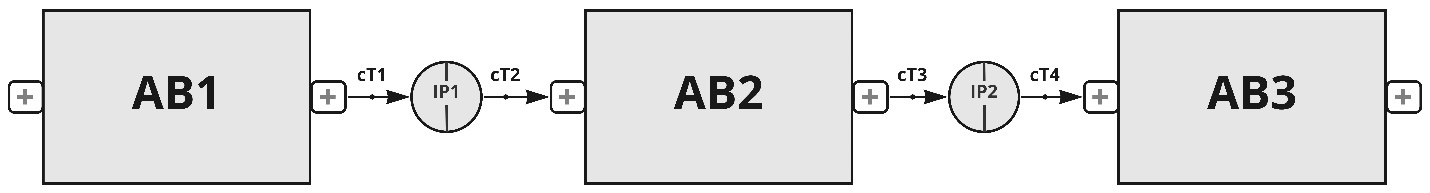
\includegraphics[width=1\textwidth]{img/IMFmanual-img045.jpg}
  \caption{A small topology between three Aspect Objects \textbf{AB1}, \textbf{AB2}, and \textbf{AB3}.}
  \label{fig:Figure 26}
\end{figure}

\begin{figure}[htb]
  \centering
  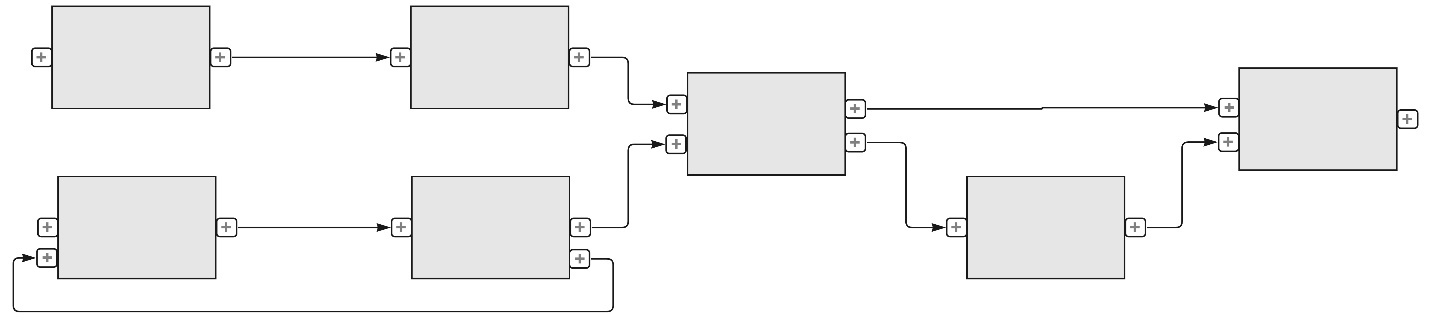
\includegraphics[width=1\textwidth]{img/IMFmanual-img046.jpg}
  \caption{A Topology.}
  \label{fig:Figure 27}
\end{figure}

Topologies can be created in all aspects. The intuition about what they represent is given in \autoref{tab:Table 15}. In this
version, only Function, Product, and Installed is considered.

\begin{table}[htb]\centering\caption{Aspect Topologies and their interpretation.}\label{tab:Table 15}
  \begin{supertabular}{|m{1.2962599in}|m{4.06286in}|m{0.8073598in}|}
    \hline
    {\bfseries Aspect Topology} &
    \textbf{Intuition} &
    {\bfseries Color}\\\hline
    {\bfseries Function Aspect Topology} &
    \textit{The Function Aspect Topology is about how Media is intended to stream between Function terminals.} &
    Yellow\\\hline
    {\bfseries Product Aspect Topology} &
    \textit{The Product Aspect Topology is specifying how artifacts shall be connected to carry }\textit{the medium }\textit{between Product terminals.} &
    Cyan\\\hline
    {\bfseries Location Aspect Topology} &
    \textit{Not used} &
    Magenta\\\hline
    {\bfseries Installed Aspect Topology} &
    \textit{The Installed Topology is documenting how the installed artifacts are connected to provide for streams between
      Installed terminals.} &
    { Dark Blue}\\\hline
  \end{supertabular}
\end{table}

\section{Combining Breakdowns and Topologies}
Combining the Breakdowns and Topologies is a powerful modelling feature. A visual of this
is given in \autoref{fig:Figure 28}. To the right, the Breakdown is shown as a tree structure. To the left, this is shown in another way as repeated zoom-ins. Here, the partOf relation is implicitly given as the dark grey child Aspect
Objects is seen as a containment and decomposition, as discussed in \autoref{ch:Section 4.4}, of the light grey parent Aspect
Object.

The left-hand side of \autoref{fig:Figure 28} is often referred to as a `Block views' and shows the Topology between the child
Aspect Objects. Notice how the Topology starts as inputs and ends as outputs from the parent Aspect Objects'
Terminals. This is a powerful mechanism that makes us able to connect streams, as discussed in \autoref{ch:Section 4.5}, across
different abstraction levels in our Breakdown.

\begin{figure}[htb]
  \centering
  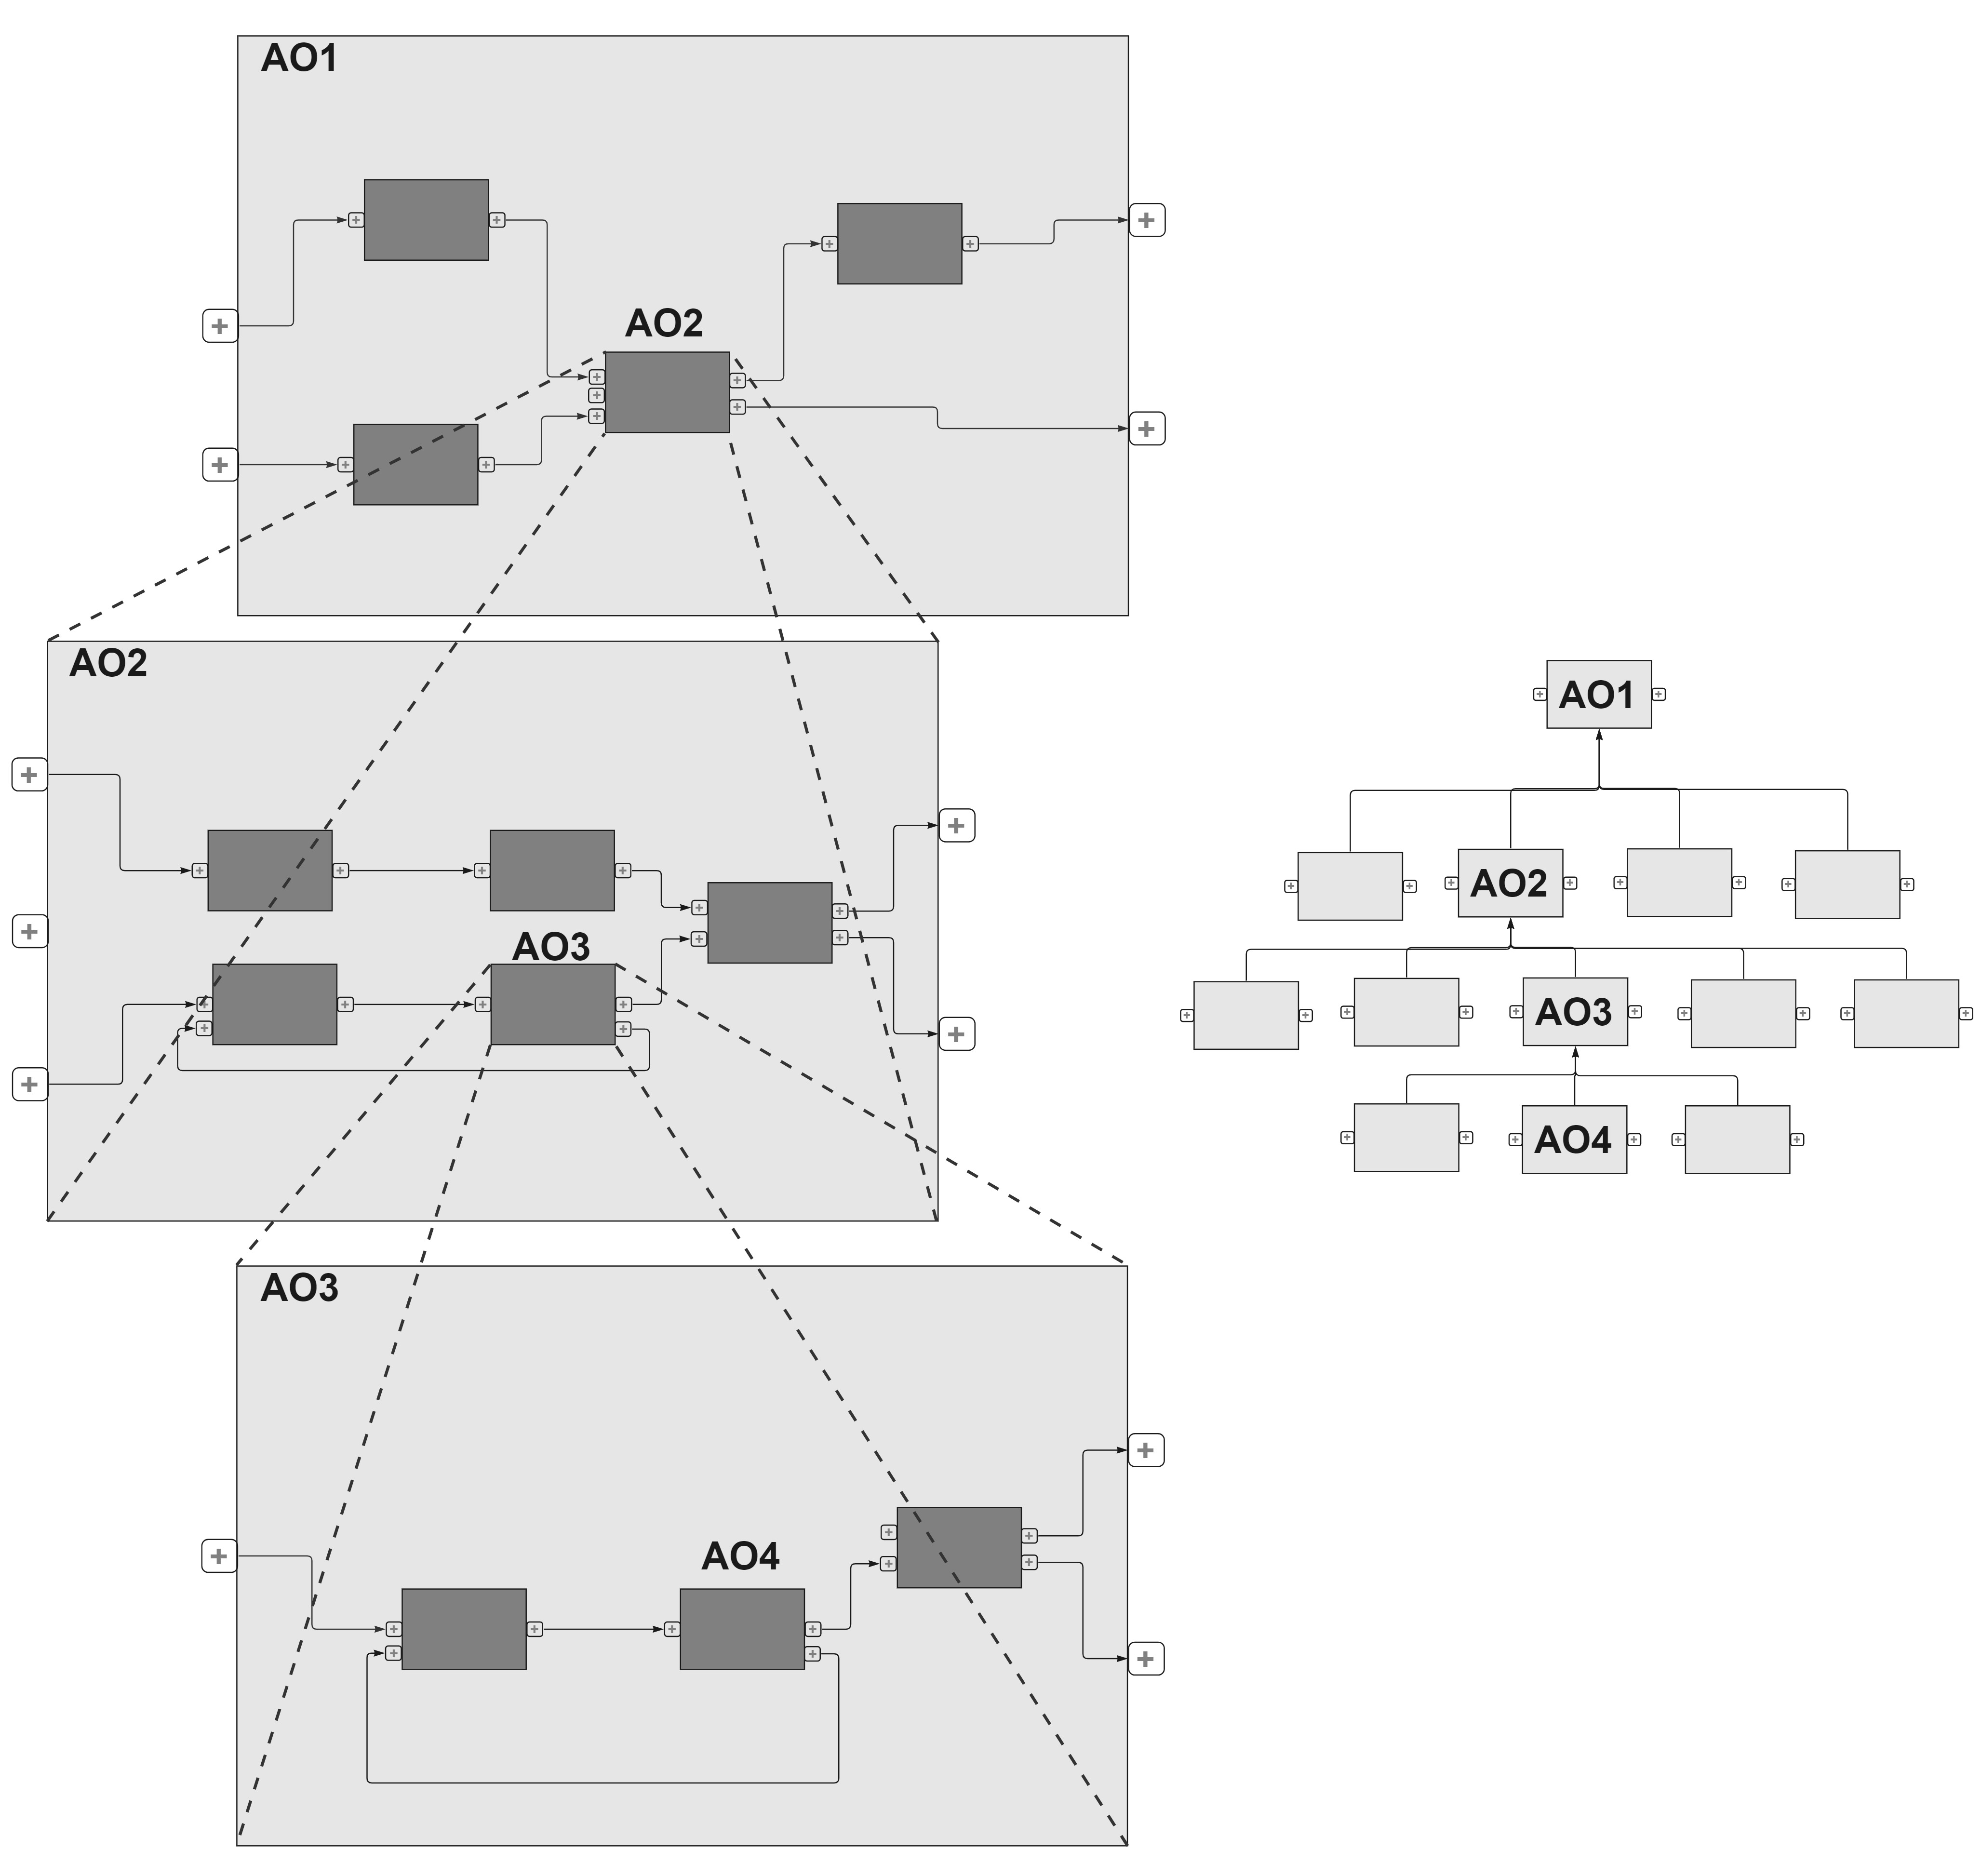
\includegraphics[width=1\textwidth]{img/IMFmanual-img047.jpg}
  \caption{Combination of Breakdown and Topology.}
  \label{fig:Figure 28}
\end{figure}

\section{Types}
An \emph{IMF type} (in this section also just called \emph{type}) is a construct from
which IMF objects are created. An object created from a type is called an \emph{instance}, and the operation of
creating an instance by using a type is called \emph{instantiation}. An instance of a type must follow the pattern
specified by the type, this means that the instance must also state the facts stated for the type, including
attributes and relations. Parts of the pattern that a type specifies may be mandatory or optional. Note that there
are also values set on the type, typically metadata such as its name, that is not part of the pattern that the
instances of the type must follow.

The purpose of types is threefold:

\begin{enumerate}
  \item Standardization
  \item Support reuse and avoid duplication of work
  \item Classification
\end{enumerate}
There are 5 kinds of types in the IMF language: Element type, Block type, Terminal type, Attribute type, and Attribute
group type. Block types, and Terminal types and Attribute types specify patterns for Blocks, Terminals, and
Attributes, respectively. An Attribute group type is a convenient collection of Attributes that is collected to a
group for ease of reuse for different types. A Terminal type may specify a Medium, a Direction (e.g., Input or Output
Terminal) and a set of Attributes. A Block type may specify a set of Terminals, and a set of Attributes. Block types
and Terminal types, which collectively are called Element types, may additionally specify a specific Aspect, a
specific notation, e.g., RDS code, and a (graphical) symbol. See \autoref{fig:Figure 29}. The Type construct may be implemented in
different ways; these are discussed below.

\subsection{Formal definitions}

\begin{figure}[htb]
  \centering
  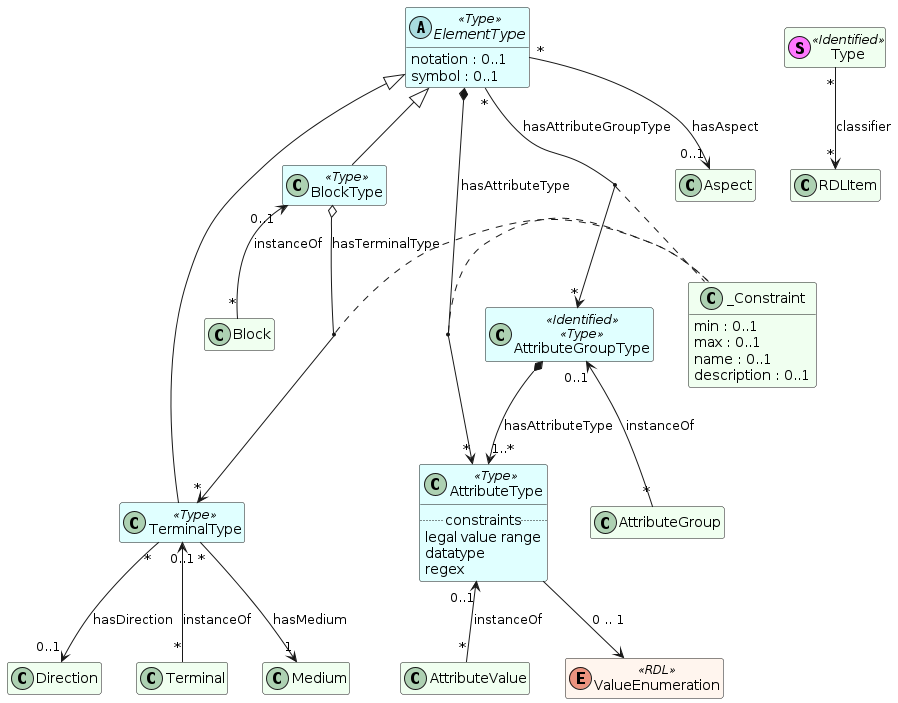
\includegraphics[width=6.2285in,height=4.87899in]{img/IMFmanual-img048.png}
  \caption{Types}
  \label{fig:Figure 29}
\end{figure}

{\itshape
Types are represented in the IMF language as objects, and the relation instanceOf is used to represent the
instantiation relationship between an instance and the type it is created from.}

\textit{All Types }\textit{may specify an arbitrary set of classifiers whose values are typically resources from reference data
  libraries (RDLs), i.e., reference data.}

\textit{An AttributeType is a type for AttributeValues. It should state a classifier that is the property of the
  instantiating AttributeValue. Additionally, an AttributeType may state different constraints that constrain the
  permissible values for an instantiating AttributeValue. }\textit{The constraints themselves are not part of the pattern that instances of the Attribute type must follow,
  i.e., the instantiating AttributeValues should not contain the constraints. A constraint may limit the permissible
  values for an AttributeValue by specifying a list of legal values, legal datatype, and/or regular expression. Other
  kinds of constraints may be possible depending on the implementation of types.}

{\itshape
  An AttributeGroupType specifies a set of attributes, via hasAttributeType relationships to AttributeTypes. An
  AttributeGroupType must be related to at least one AttributeType.}

{\itshape
  An ElementType is either a BlockType or a TerminalType. An ElementType may state a notation, which may be any value,
  but typically a string, and a symbol that is used to visualize instances of the type. An ElementType may also state
  an Aspect using the hasAspect relation. An ElementType specifies a set of attributes, via hasAttributeType
  relationships to AttributeTypes, or via hasAttributeGroupType relationships to AttributeGroupTypes. These
  relationships must be constrained by cardinality constraints that specify the minimum and maximum number of required
  instances required of the related types. Optional attributes are specified for a type are specified by setting
  minimum cardinality to 0. Mandatory attributes are specified by setting a number greater than 0.}

{\itshape
  A TerminalType is an ElementType and is a type for Terminals. It may state a Medium and a Direction.}

{\itshape
  A BlockType is an ElementType and a type for Blocks. It may specify a set of Terminals, via hasTerminalType
  relationships to TerminalTypes. The relationships must be constrained by cardinality constraints.}

\textit{instanceOf is a relation between an object and a type and expresses that the object is an instance of the type. This
  statement is true if the object fulfills the constraints expressed for the type. This means that the object must
  state all fields stated for the type, and that the object must state all the mandatory attributes stated for the type
  and abide by the constraints stated on the AttributeTypes stated for the Type. }



\paragraph{Discussion on different implementations of types}

Types are meant to serve a range of purposes. This makes it relevant to implement the functionality of types with
different languages.

\begin{itemize}
  \item A type can be represented as a \emph{prototypical }object\emph{. }This is the format described above.
        Instances of the type are created from the type by ``copying the type'' and further detailing the copy according to
        the constraints stated on the type.
  \item A type can be represented as a (OWL) class, whose members are the instances of the type. A class implementation
        is useful for classifying objects according to a set of types, and for identifying specialization/generalization
        relationships between types.
  \item A type may be represented as a (SHACL) constraints, where the instances of the type are objects that satisfy the
        constraints. This implementation is useful for (automatically) verifying that the stated instances of a type follow
        the requirements stated by the type.
  \item A type may be represented as a (OTTR) template, where the instances of the type are created by instantiating the
        template. This implementation is useful for easily creating type instances with a certain guarantee of correctness.
\end{itemize}
We anticipate that the IMF framework will provide translations between the prototypical format to the other formats.